\section{Introduction}

The Architectures part of this thesis was introduced, in \Cref{chap:data_oriented_perspective}, as the part in which the standardization of an individual Digital Twin's data architecture is addressed concretely, through the design of a data platform tailored to the requirements of the applications it serves. This chapter presents that instantiation, developed within AGRITECH, Italy's National Research Centre for Agricultural Technologies, funded under the National Recovery and Resilience Plan (PNRR).\footnote{\url{https://agritechcenter.it}} Precision agriculture provides a particularly demanding testbed for a data-oriented design: agricultural monitoring routinely combines structured sensor time series, satellite raster imagery, and unstructured field observations, produced at rates ranging from sub-hourly weather readings to seasonal crop surveys, and consumed by stakeholders with markedly different backgrounds and objectives, from agronomists to machine-learning researchers.

Within AGRITECH, Spoke~3 is concerned with enabling technologies and sustainable strategies for the management of agricultural systems and brings together six research partners, each pursuing distinct, independently defined research activities: precision irrigation, robotics-based field monitoring, geospatial analysis, and predictive modelling of agronomic phenomena, among others. Left to develop independently, these activities would reproduce, in miniature, precisely the fragmentation this thesis warns against: overlapping data sources collected and stored in incompatible formats, with no common ground for their later integration or reuse. At the same time, imposing a single, project-specific data architecture on all six partners would misrepresent the diversity of their objectives and disciplines, echoing the same tension between domain specificity and standardization discussed throughout \Cref{chap:digital_twins,chap:data_oriented_perspective}.

The response adopted within AGRITECH, and presented in this chapter, is a \emph{domain-level} data platform: infrastructure and a shared conceptual schema designed around the recurring concepts of the precision agriculture domain as a whole, rather than around the specific application any one partner is pursuing. This distinction between the \emph{domain level} (i.e.,  the concepts, rules, and requirements shared across a class of applications) and the \emph{application level} (i.e. the implementation solving a specific problem within a domain, such as scheduling irrigation for a given crop) recurs throughout this chapter, and gives the resulting platform its defining property: partners retain full autonomy over their application-level processes and analyses, while sharing a common substrate for how their data is ingested, represented, and stored.

\Cref{sec:dataplat-characterization} reports the methodology followed to characterize the data relevant to the AGRITECH domain, and the resulting characterization. \Cref{sec:dataplat-refarch} derives, from these requirements, a reference architecture for the data platform and the conceptual schema used to represent the domain. \Cref{sec:dataplat-implementation} describes the concrete implementation of the platform. Finally, \Cref{sec:dataplat-discussion} assesses the platform against the six partners' use cases and situates the contribution within the broader argument of this thesis.

\section{Characterizing Precision Agriculture Data}
\label{sec:dataplat-characterization}

Designing a data platform around the needs of a domain, rather than around a single application, first requires that domain's data to be characterized independently of any one partner's perspective. This characterization of data was achieved through an iterative process aimed at characterizing the data produced, and consumed by the partners.

\subsection{Requirements identification}

The first step in requirement gathering was conducted through a one-to-one meeting with each of the six partners, in which each one of them was asked to present their research activity in terms of requirements, goals and expected methodology, trying to build a first, broad view of the different types of data involved.
Then, each partner was asked to participate in a more specific survey which tried to characterize the data involved in their research activities, in order to identify the data they produce and consume, and the processing capabilities they require.

Considering the nature of the data involved, the survey aimed at describing the data in terms of some of the notorious big data "V"s~\cite{DeMauro2016}, specifically: variety, volume, veracity and velocity. Variety refers to the different types of data involved, from structured sensor readings to unstructured field observations; volume refers to the scale of the data, from individual sensor readings to multi-gigabyte satellite acquisitions; veracity refers to the quality and consistency of the data, which is often collected and shared manually by domain experts. Velocity refers to the temporal reference of data; similarly, questions were asked to identify the spatial reference of data, as virtually all data of interest is tied to a specific location other than a specific point or interval in time.

Once the survey was completed, a second and last round of one-to-one meetings was conducted to clarify any remaining ambiguities and further discuss the results of the survey.

This process surfaced two findings that shaped the resulting design. First, at the level of the domain as a whole, the six partners' projects were found to be comparatively volatile -- research objectives and data needs evolved over the course of the project rather than remaining fixed -- and, initially, largely non-communicating, with data shattered across incompatible formats and no shared ground for interoperability even where partners' activities overlapped, such as in crop monitoring or the use of satellite imagery, as shown in \Cref{fig_agritech_plat}. Second, at the level of the data itself, four recurring characteristics emerged across partners:

\begin{itemize}
    \item \textbf{Variety}: data types spanned vector data (e.g., parcel boundaries and robot trajectories), raster and multispectral imagery (e.g., satellite and drone-acquired images), and sensor time series (e.g., soil moisture and weather readings), with little consistency in format even across partners working on related problems.
    \item \textbf{Volume}: data scale ranged from individual sensor readings, at the byte scale, to multi-gigabyte drone missions and satellite acquisitions, with no single storage or processing solution well suited to the full range.
    \item \textbf{Veracity}: a substantial share of the data was collected and shared manually by domain experts rather than acquired automatically, introducing quality and consistency issues that an architecture designed only around automated sensor feeds would not anticipate. Furthermore, some data was produced by third-party sources, such as satellite imagery providers or other research institutions, over which the partners had no control and whose quality could not be guaranteed.
    \item \textbf{Velocity}: data was produced and consumed at different rates, from sub-hourly weather readings to seasonal crop surveys and weekly satellite acquisitions, with no single processing solution well suited to the full range.
    \item A strong \textbf{spatio-temporal connotation}: virtually all data of interest was tied to a specific location and a specific point or interval in time, making spatial and temporal reference first-class requirements rather than incidental metadata.
\end{itemize}

\begin{figure}[h!]
    \centering
    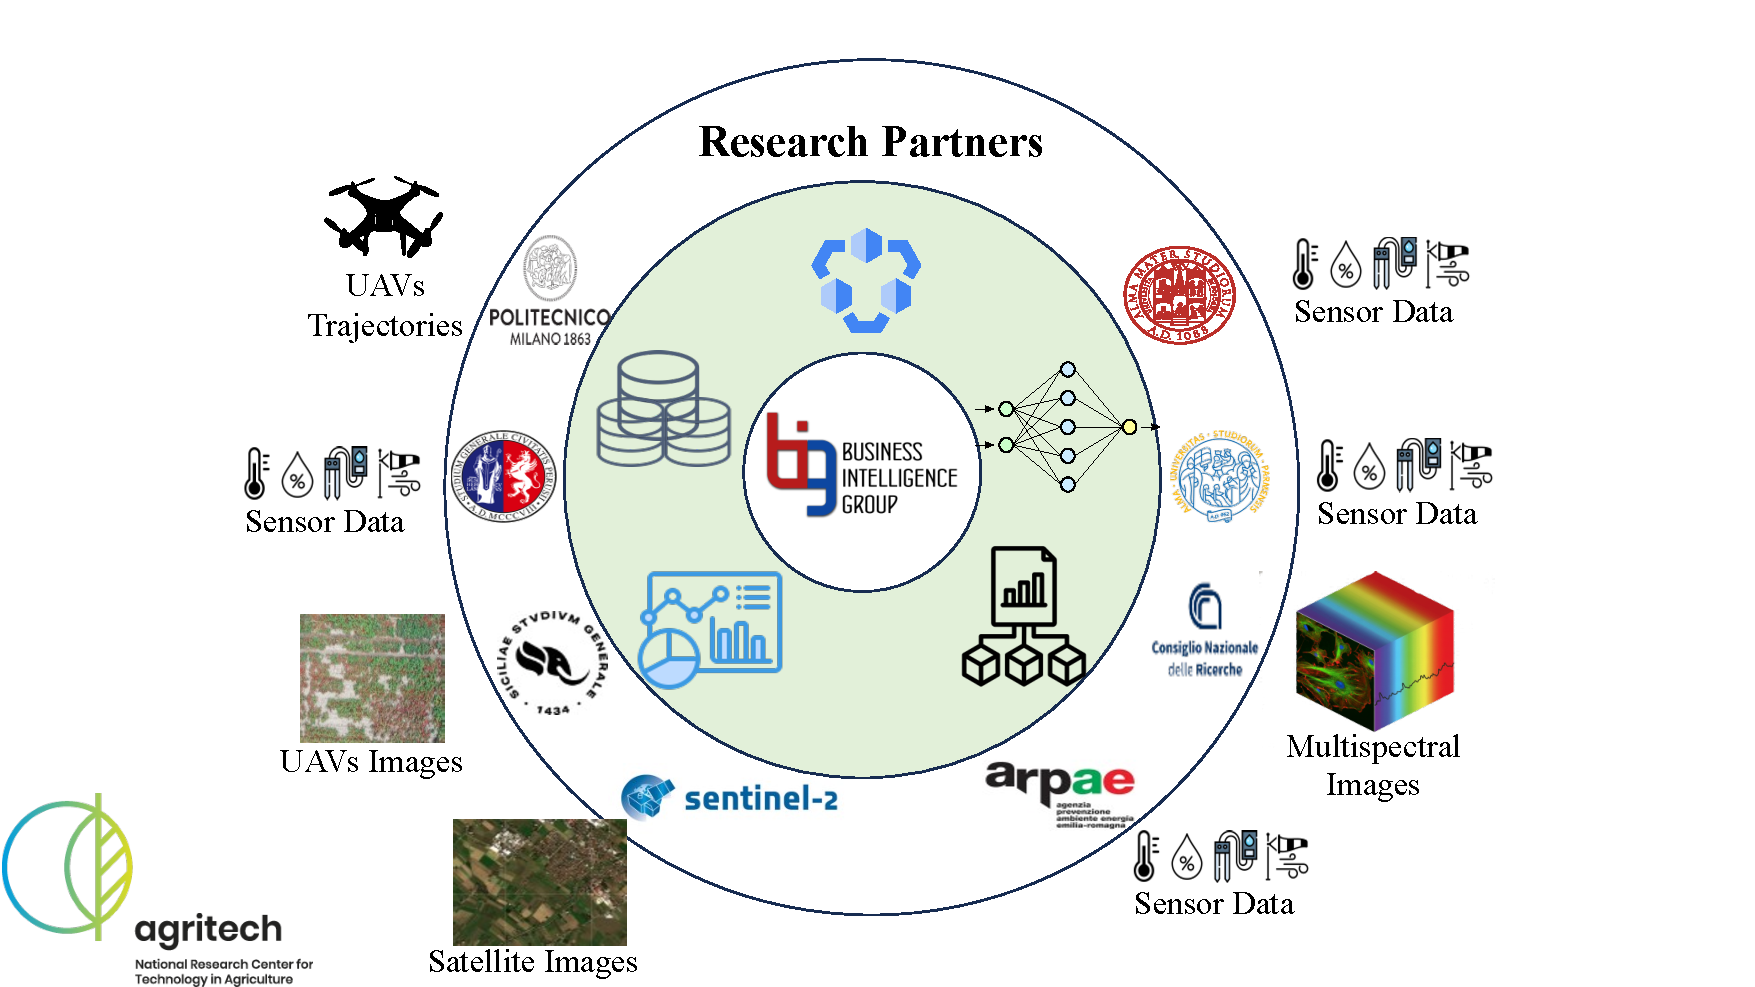
\includegraphics[scale=0.5]{parts/architectures/images/agritech_arch.pdf}
    \caption{Conceptual representations of the nature of the research partners' data.}
    \label{fig:agritech_plat}
\end{figure}

\subsection{Terminology Analysis}

Requirements elicited directly from six partners, however numerous, cannot be assumed to cover the concepts recurring across the precision agriculture domain at large; a platform designed only around them would risk being an accurate model of these six projects rather than of the domain they belong to. To mitigate this risk, the requirements above were cross-checked against an independent analysis of domain terminology, obtained by scraping the accepted papers of the last four editions (2020--2023) of the European Conference on Precision Agriculture (ECPA), and ranking the 1300 most frequent terms out of the 3000 extracted.

This analysis served two purposes. First, it confirmed the centrality of the same data-oriented characteristics identified through the partner interviews: among the ten most frequent terms in the corpus, \emph{sensor}, \emph{data}, \emph{multispectral}, and \emph{image} directly denote the variety of data types just discussed, while \emph{management} and \emph{machine learning} point to the processing and analytics needs the platform is expected to support. Second, and more directly relevant to the schema presented in \Cref{sec:dataplat-refarch}, it distinguished terms denoting real-world entities or measurable properties worth representing explicitly in a conceptual schema (e.g., \emph{crop}, a physical entity, and \emph{yield}, a measurable property of a crop) from terms denoting abstract fields, techniques, or research areas (e.g., \emph{precision agriculture} or \emph{machine learning} itself), which a data-oriented conceptual schema is not intended to represent.

Taken together, these two analyses characterize the data this platform is designed to support along four axes -- variety, volume, veracity, and spatio-temporal reference -- and identify a first candidate set of domain concepts worth representing explicitly. The following sections derive from this characterization, in turn, a reference architecture for the platform (\Cref{sec:dataplat-refarch}) and, building on it, a domain-level data model representing these concepts (\Cref{sec:dataplat-datamodel}).

\section{A Reference Architecture for the Data Platform}

This section describes a reference architecture for the AGRITECH data platform, derived from the characterization of the domain's data in \Cref{sec:dataplat-characterization}. The architecture is organized around independent, composable modules, each responsible for one stage of the data life cycle, from ingestion to exploitation. The following sections describes the conceptual model of the platform (\Cref{sec:dataplat-refarch}) and then discuss technical implementations on an on-premises cluster (\Cref{sec:dataplat-implementation}).

\subsection{A conceptual view}
\label{sec:dataplat-refarch}


\begin{figure}[htbp]
    \centering
    \makebox[\textwidth][c]{%
        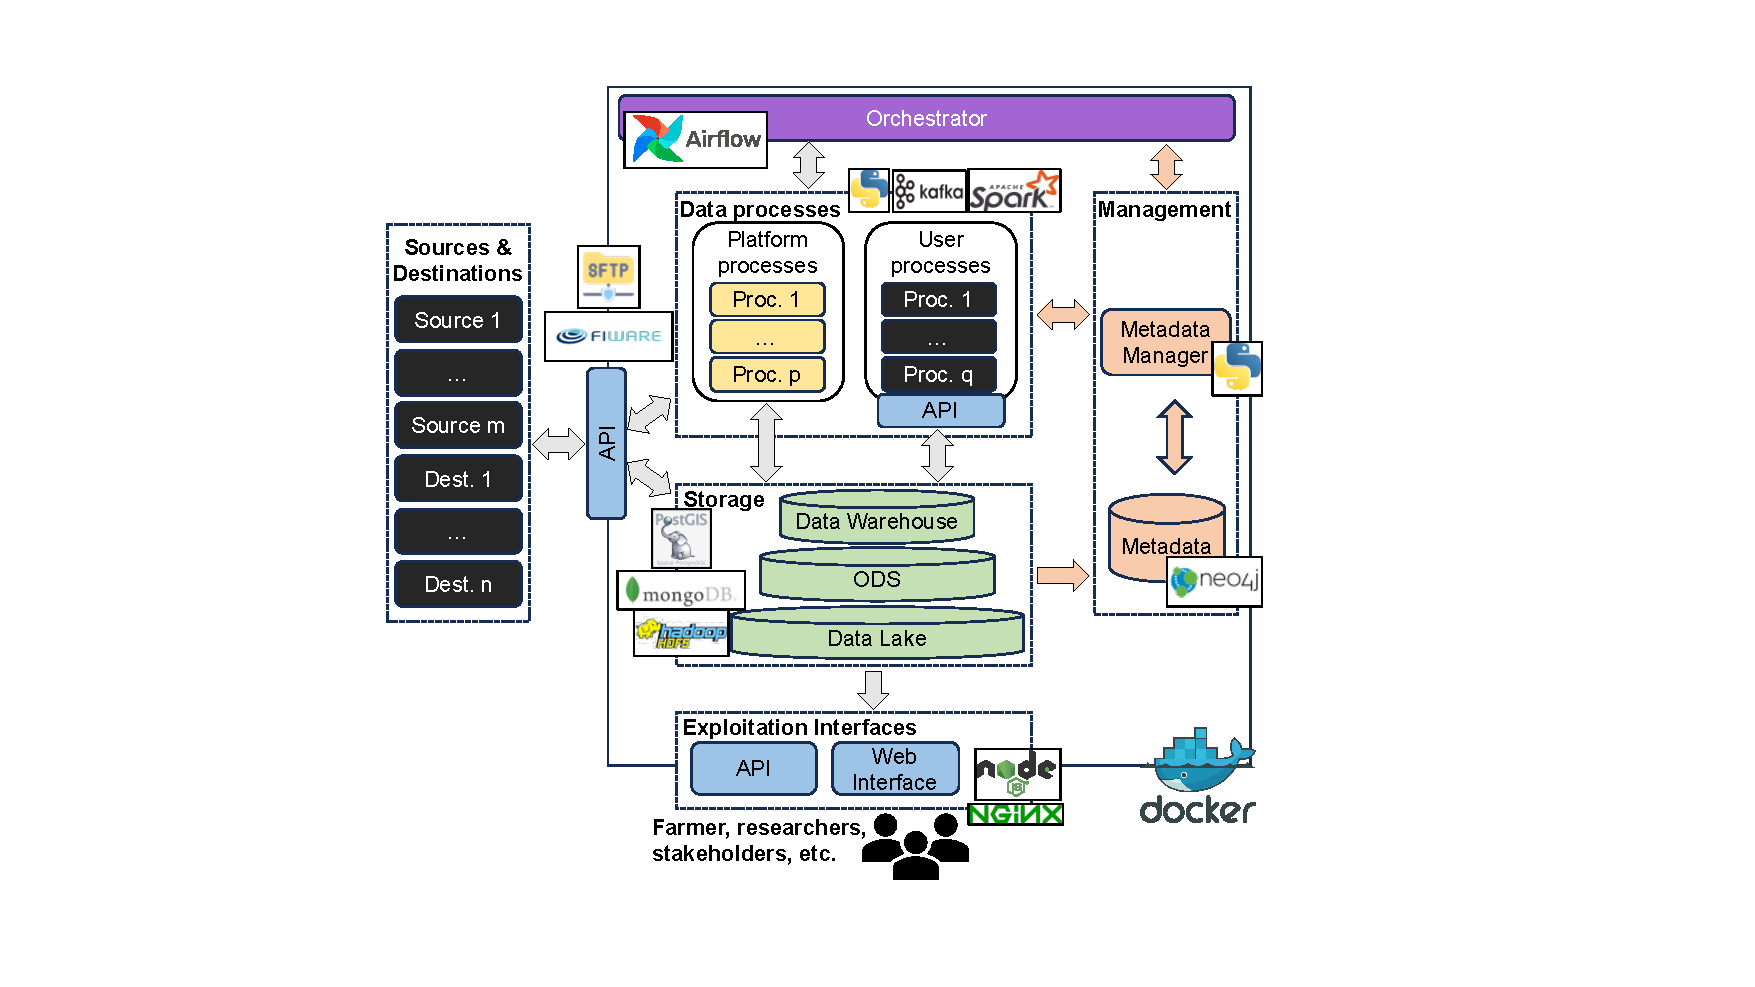
\includegraphics[trim=0pt 45pt 45pt 35pt, clip, width=1.15\textwidth]{parts/architectures/images/agritech_platform.pdf}%
    }
    \caption{A reference data architecture for the AGRITECH data platform, organized around independent, composable modules.}
    \label{fig:agritech_architecture}
\end{figure}

The variety, volume, veracity, and spatio-temporal character of the data identified in \Cref{sec:dataplat-characterization} motivate an architecture organized around independent, composable modules, each responsible for one stage of the data life cycle, from ingestion to exploitation (fig:dataplat-architecture).


\begin{itemize}
    \item \textbf{Ingestion} is responsible for admitting raw data into the platform from heterogeneous sources -- relational or NoSQL databases, files, or third-party APIs such as those providing satellite-derived vegetation indices -- directly reflecting the variety identified above. Three ingestion modes are distinguished: \emph{push} ingestion, in which sources continuously stream data into the platform as it is produced (e.g., a robot updating its GPS trajectory); \emph{pull} ingestion, in which the platform periodically retrieves data from an external source on a fixed or ad-hoc schedule (e.g., downloading a weekly satellite acquisition); and \emph{manual} ingestion, for data collected and uploaded directly by domain experts -- the mode most exposed to the veracity concerns discussed above.
    \item \textbf{Storage} persists both raw and processed data across repositories suited to their variety and volume. Following the standard data-warehousing distinction, the architecture separates \emph{operational} data, addressing the immediate, short-term needs of a process (e.g., the latest sensor reading), from \emph{strategic} data, supporting longer-term, historical analysis (e.g., multi-year pest trends). A data lake accommodates raw data in its native format, irrespective of structure; databases accommodate data conforming to a specific model (relational, document, or graph); and, where reconciled historical analysis is required, an operational data store or a data warehouse accommodates data integrated across sources.
    \item \textbf{Data processes} transform operational data into knowledge of increasing strategic value, spanning both \emph{streaming} processing, producing results within seconds of data arrival, and \emph{batch} processing, operating over larger collections with a longer completion horizon. This module is discussed further below.
    \item \textbf{Management} oversees the data life cycle through profiling and metadata management, addressing the provenance and quality properties that the veracity concerns identified above make especially relevant.
    \item \textbf{Exploitation} governs how raw data or the knowledge derived from it is consumed by its end users, be they developers, domain experts, or other processes running on the platform. Because these users differ significantly in technical background, the architecture supports multiple fruition endpoints, from programmatic APIs to ready-made web interfaces.
    \item An \textbf{orchestrator} coordinates data and management processes into larger, repeatable pipelines, sequencing dependent tasks and scheduling their recurring execution.
\end{itemize}

The distinction drawn above between platform and user processes deserves closer attention, since it is what allows the platform to remain agnostic to the internal implementation of each partner's application, the same property \Cref{chap:data_oriented_perspective} attributed to a Digital Twin Platform with respect to the Digital Twins it hosts, applied here one level down, to the individual processes it hosts.

\emph{Platform processes} are internal to the platform itself, and are typically responsible for producing or maintaining data of shared value across partners. During the requirements gathering phase, it emerged that some data was used by almost every stakeholder: for instance, externally sourced reference data such as satellite imagery produced by Copernicus\footnote{\url{https://dataspace.copernicus.eu/}}, and weather measurements collected by the Regional Agency for Prevention, Environment and Energy of Emilia-Romagna (ARPAE)\footnote{\url{https://www.arpae.it/it}}. Because they are developed and maintained as part of the platform, platform processes are granted direct, trusted access to its storage layer, and ensure that the resulting data conforms to the platform's representation standards, giving all partners a single representation to consume rather than one each (and avoiding the duplicated storage costs of every partner keeping its own copy). Typical platform processes include \emph{data ingestion} (admitting raw data into the platform), \emph{data cleaning} (correcting errors and inconsistencies in the data), and \emph{data integration} (reconciling data from multiple sources into a single representation).

\emph{User processes}, by contrast, are applications deployed and controlled by individual partners, hosted on the platform but developed independently of it and of one another. Consistently with the modularity and independence expected of a data platform \cite{francia2025process}, user processes are treated as black boxes: rather than being granted direct access to the platform's storage, they interact with it exclusively through well-defined APIs. This has a double effect: a partner is free to implement, modify, or replace their own processes without affecting the platform or any other partner's activity, while the platform, in turn, does not need to know how a given user process is implemented internally, only that the data it consumes and produces through these shared interfaces conforms to the same representation standards platform processes are held to. User processes typically implement application-specific pipelines, collecting and transforming the data a given application requires; the same API layer that isolates them from the platform's internals also ensures that the data they produce can, in turn, be consumed by other partners' applications, and vice versa.
-
This separation between a small set of trusted platform processes and an open-ended, partner-defined set of user processes is what allows the platform to scale to a growing and evolving set of partners and applications: what must remain uniform is not the software each process runs, but the representation of the data it exchanges with the platform, discussed next in \Cref{sec:dataplat-datamodel}.

\subsection{Technological Stack}
\label{sec:dataplat-implementation}

The modules identified in \Cref{sec:dataplat-refarch} were implemented on an on-premises cluster, containerized through Docker\footnote{\url{https://www.docker.com/}} in Swarm mode, a choice motivated by cost, long-term availability beyond the project's own duration, and the modularity and fault tolerance a containerized, orchestrated infrastructure affords over a bare-metal deployment. The remainder of this section maps each module of the reference architecture onto the specific technology used to implement it.

\emph{Ingestion} is implemented around FIWARE\footnote{\url{https://www.fiware.org}} and, specifically, its Orion Context Broker, which exposes the NGSI-LD API as the platform's single entry point for context data. Real-world objects are represented as entities conforming to Smart Data Models, each required to carry, at minimum, an identifier, a type, a human-readable name, and the identifier of the owning partner; representative entity types instantiated for AGRITECH include \texttt{Device}, \texttt{AgriFarm}, \texttt{AgriParcel}, \texttt{AgriTree}, \texttt{Camera}, and \texttt{Task}. The three ingestion modes distinguished in \Cref{sec:dataplat-refarch} map directly onto this implementation: push ingestion is realized through Orion's creation and update APIs, pull ingestion through internal processes retrieving data on a schedule, and manual ingestion through SFTP file transfer for partners uploading data directly.

\emph{Storage} is realized as a data lake combining HDFS \cite{white2012hadoop}, holding raw, high-volume data such as satellite archives and robot mission logs, with MongoDB, holding the semi-structured, NGSI-LD-conformant entities produced by the ingestion layer together with their history. The two repositories accordingly reflect the operational/strategic distinction of \Cref{sec:dataplat-refarch}: HDFS as the substrate for large-scale batch processing, MongoDB as the up-to-date, queryable view of the platform's entities.

\emph{Data processes} are supported through Apache Kafka\footnote{\url{https://kafka.apache.org/}} \cite{shapira2021kafka} for streaming and Apache Spark\footnote{\url{https://spark.apache.org/}} \cite{chambers2018spark} for batch workloads. Platform processes exploit this combination in different ways: recurring platform processes retrieve and reconcile externally sourced data, such as ARPAE's weather archives or Copernicus Sentinel-2 imagery, storing the raw archives in HDFS and the resulting SDM-conformant entities in MongoDB; a further platform process historicizes every entity created or updated in Orion by subscribing to the corresponding events, publishing them as a Kafka stream, and persisting them to MongoDB, partitioned by owning partner.

The \emph{orchestrator} is implemented with Apache Airflow,\footnote{\url{https://airflow.apache.org/}} adopted in place of the originally considered Oozie for its Python-based workflow definitions and its web-based monitoring interface, both directly relevant to a platform whose processes are, in large part, contributed and maintained by external partners rather than by the platform's own developers.

Finally, \emph{exploitation} is realized through a web application, served by Nginx\footnote{\url{https://www.nginx.com/}} with a Node.js\footnote{\url{https://nodejs.org/}} backend, centred on an interactive map that renders georeferenced entities by type and exposes their attribute history, alongside a hierarchical view for navigating the platform's entities by owner and type. Programmatic access is provided through APIs specified according to the OpenAPI standard, ensuring that the same representation standards enforced at the level of ingestion and storage extend to how the platform's data is ultimately consumed.

\section{Towards a Domain-Level Data Model}
\label{sec:dataplat-datamodel}

The reference architecture presented in \Cref{sec:dataplat-refarch} standardizes how data is acquired, stored, and made available across the platform's modules, irrespective of what that data represents. As discussed in \Cref{chap:data_oriented_perspective}, however, standardizing this infrastructural layer does not by itself guarantee that the data flowing through it is represented consistently, or that its meaning is preserved as it moves from one partner's application to another's. This section addresses that complementary concern: how the entities relevant to the AGRITECH domain should themselves be represented, so that partners' data can be integrated rather than merely co-located.

\subsection{FIWARE Smart Data Models}

The terminology analysis in \Cref{sec:dataplat-characterization} identifies \emph{what} concepts a shared representation of the domain should cover, but not \emph{how} such concepts should be digitally modelled for effective transmission and storage; neither the literature nor domain dictionaries such as AGROVOC\footnote{\url{https://www.fao.org/agrovoc/}} address this second question. A natural starting point is the FIWARE foundation, which supports the sharing of information across several sectors, including precision agriculture, sensing, and smart cities.\footnote{\url{https://www.fiware.org}} Within FIWARE, real-world objects -- a farm, a parcel, a sensor -- are mapped into digital entities described by \emph{Smart Data Models} (SDM), each composed of a schema defining the entity's attributes and their types, a human-readable specification, and example payloads. Smart Data Models are grouped into subjects belonging to one or more domains, where a domain corresponds to an industrial sector; they are public, free to use, modify, and share, and are explicitly intended as blueprints for real-world applications.

Despite this, adopting Smart Data Models directly, as a shared representation for the platform, would not resolve the fragmentation this chapter is concerned with. Smart Data Models present four limitations in this respect. First, they are designed to be application- and transmission-oriented, which limits the extent to which the data they describe can be extended and integrated into higher-level knowledge. Second, they provide no unified interface for accessing and manipulating the data they describe, so that a data lake populated directly with SDM-conformant entities risks becoming, in practice, a data swamp in which the necessary data is difficult to locate even when present. Third, they exhibit intra- and inter-domain inconsistencies and redundancy: the same real-world concept can exist in different domains with different semantics or attributes -- a greenhouse, for instance, is modelled as a \texttt{Building} in the Smart City domain but as a first-class \texttt{AgriGreenhouse} in the Precision Agriculture domain\footnote{\url{https://smart-data-models.github.io/dataModel.Building/Building/} and \url{https://smart-data-models.github.io/dataModel.Agrifood/AgriGreenhouse/}} -- and the same concept can be modelled in more than one way even within the same domain, as when a sensor measurement is represented directly as an attribute of a \texttt{Device} in one case and as a first-class \texttt{DeviceMeasurement} in another.\footnote{\url{https://smart-data-models.github.io/dataModel.Device/Device/} and \url{https://smart-data-models.github.io/dataModel.Device/DeviceMeasurement/}} Fourth, distinct notions are sometimes aggregated within a single concept -- for instance, a sensor and its measurement within the same \texttt{Device} -- to keep the resulting payloads compact and efficient to transmit (e.g., over MQTT); the same tendency to aggregate distinct notions for the sake of compactness has been reported in ontologies developed for the agricultural domain more generally \cite{jonquet2018agroportal,hu2011agont}.

These limitations motivate defining an integrated, domain-level conceptual schema, rather than adopting Smart Data Models as they stand: the goal is to map the entities exposed at the level of individual sources and applications onto a restricted set of higher-level concepts, atop which analytics can be carried out uniformly across partners. As a first step in this direction, the entities and attributes identified across the six partners' projects were matched, where possible, against existing Smart Data Models (\Cref{tab:sdm-mapping}). This mapping exercise showed that (i) not every entity has a ready SDM counterpart, so that new models must sometimes be created or existing ones extended; (ii) more than one SDM representation is occasionally available for the same entity, requiring an explicit choice between them; and (iii), most importantly, that the entities involved could be generalized into a small number of recurring notions -- agents, measurements, tasks, and environments -- which the domain-level conceptual schema presented next takes as its starting point.

\begin{table}[h!]
\centering
\caption{Mapping selected domain concepts to FIWARE Smart Data Models.}
\label{tab:sdm-mapping}
\begin{tabular}{lll}
\toprule
\textbf{Term} & \textbf{FIWARE SDM} & \textbf{Standardized Concept} \\
\midrule
Robot, Weather station & Device & Agent \\
AI process & -- & Agent \\
Temperature, Humidity & Device, DeviceMeasurement & Measurement \\
Weeding, Monitoring & -- & Task \\
Emilia Romagna & -- & Environment \\
Parcel & AgriParcel & Environment \\
Farm & AgriFarm & Environment \\
\bottomrule
\end{tabular}
\end{table}

\subsection{A Domain-Level Conceptual Schema}

The terminology analysis in \Cref{sec:dataplat-characterization} identified candidate domain concepts but not the relationships among them, nor a criterion for deciding which concepts belong in a shared schema and which are better left to individual applications. The conceptual schema addresses both questions, organizing the identified concepts into four zones (\Cref{fig:dataplat-schema}).

\begin{figure}[h!]
    \centering
    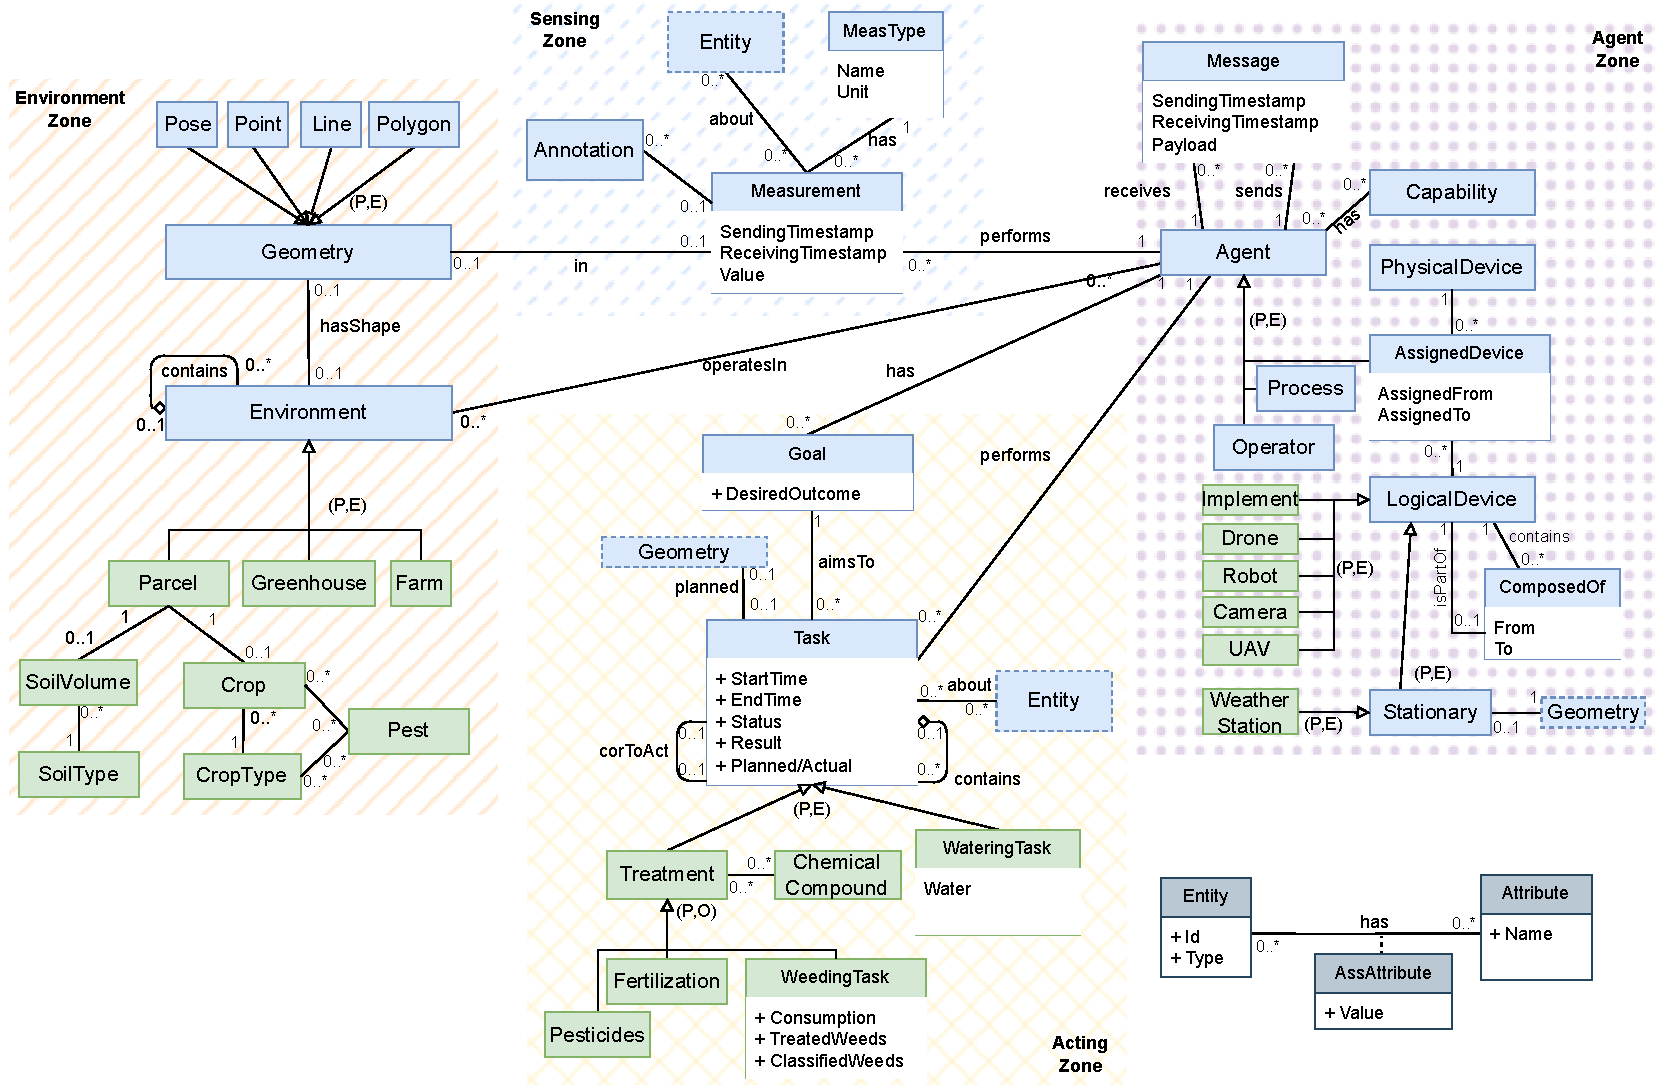
\includegraphics[scale=0.5]{parts/architectures/images/agritech_dm.pdf}
    \caption{The proposed AGRITECH domain-level conceptual schema, organized into four zones: agent, environment, sensing, and acting.}
    \label{fig:dataplat-schema}
\end{figure}

The data model  schematizes the main components of Digital Twins and their conceptual organization as much as its hierarchical structure. The \emph{agent} zone represents the master data of entities that sense and act within an environment to pursue a goal: an \texttt{Operator} is a human agent (e.g., a farmer), a \texttt{Process} is an ICT agent with no physical counterpart (e.g., an AI vision system), and a \texttt{LogicalDevice} represents the role played, at a given time, by some \texttt{PhysicalDevice}: such a distinction allows, for instance, a faulty physical sensor to be replaced without altering the logical identity of the measurement point it realizes. The \emph{environment} zone represents the hierarchical, georeferenced areas in which agents operate (e.g., a farm composed of parcels). The \emph{sensing} zone represents the history of data sensed by an agent, as \texttt{Measurement}s characterized by a type, a precision, and an accuracy, and optionally annotated (e.g., a bounding box marking a detected weed within an image). The \emph{acting} zone represents the history of actions an agent undertakes, as hierarchically composed \texttt{Task}s with associated space and time dimensions, and both a planned and an executed form.

Concepts in each zone are further distinguished as either \emph{domain-agnostic} (in blue in \Cref{fig:dataplat-schema}), when generic enough to fall outside precision agriculture altogether and to be assimilated directly to the notion of a Digital Twin itself, as components recurring in a Digital Twin regardless of its domain (e.g., \texttt{Agent}, \texttt{Task}, \texttt{Measurement}), or \emph{domain-specific} (in green in \Cref{fig:dataplat-schema}), when specialized to a specific domain; in this case, the agritech setting (e.g., \texttt{Crop}, \texttt{Parcel}, \texttt{Farm} as specializations of \texttt{Environment}, or \texttt{Robot} and \texttt{WeatherStation} as specializations of \texttt{LogicalDevice}). This distinction is what makes the schema extensible to concepts not yet identified: a new domain-specific concept can be introduced as a specialization of an existing domain-agnostic one without revising the schema itself.
Similarly, the domain-agnostic concepts are intended to be reusable across domains, so that a new domain-specific concept can be introduced as a specialization of an existing domain-agnostic while still having some common ground with other domains, and without requiring a new schema to be defined from scratch.

